\section{Элементарная алгебра}

% Вспомнить о понятии окрестности точки,
% функции расстояния --- метрики (см. п. 5)

\subsection{Виды выражений}

{\bold Одночлен} {\ital (моном)} --- произведение переменных и коэффи"=циентов.

{\bold Многочлен} {\ital (полином)} --- сумма одночленов.

{\bold Двучлен} {\ital (бином)} --- многочлен из двух одночленов.

{\bold Трёхчлен} {\ital (трином)} --- многочлен из трёх одночленов.

Многочлен $P$ от одной переменной $x$ можно представить так:
% ---
$$P=\sum^{n}_{k=0}a_kx^{n-k}$$

\subsection{Квадратный трёхчлен}

Расположение корней относительно числа $p$:

\begin{sheet*}[SC|SC]
\rowcolor{table}
\bold Расположение корней & \bold Равносильно\\
\adjustbox{valign=c}{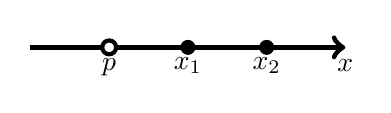
\begin{tikzpicture}[baseline={(0,0.25)}]
\draw [->,line width=2pt](-2,0) -- (2,0) node[below] {$x$};
\draw [fill=white, draw=black, line width=1.5pt] (-1,0) circle (2.5pt) node[below] {$p$};
\draw [fill=black] (0,0) circle (2.5pt) node[below] {$x_1$};
\draw [fill=black] (1,0) circle (2.5pt) node[below] {$x_2$};
\end{tikzpicture}} &
$\left\{\begin{aligned}
&D\greater 0\\
&af(p)\greater 0\\
&p\less x_0
\end{aligned}\right.$\\\hline
\adjustbox{valign=c}{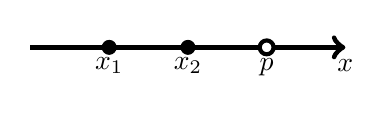
\begin{tikzpicture}[baseline={(0,0.25)}]
\draw [->,line width=2pt](-2,0) -- (2,0) node[below] {$x$};
\draw [fill=black] (-1,0) circle (2.5pt) node[below] {$x_1$};
\draw [fill=black] (0,0) circle (2.5pt) node[below] {$x_2$};
\draw [fill=white, draw=black, line width=1.5pt] (1,0) circle (2.5pt) node[below] {$p$};
\end{tikzpicture}} &
$\left\{\begin{aligned}
&D\greater 0\\
&af(p)\greater 0\\
&x_0\less p
\end{aligned}\right.$\\\hline
\adjustbox{valign=c}{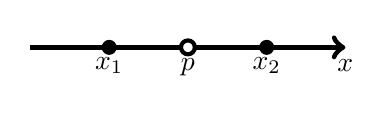
\begin{tikzpicture}[baseline={(0,0.25)}]
\draw [->,line width=2pt](-2,0) -- (2,0) node[below] {$x$};
\draw [fill=black] (-1,0) circle (2.5pt) node[below] {$x_1$};
\draw [fill=white, draw=black, line width=1.5pt] (0,0) circle (2.5pt) node[below] {$p$};
\draw [fill=black] (1,0) circle (2.5pt) node[below] {$x_2$};
\end{tikzpicture}} &
$af(p)\less 0$
\end{sheet*}

\newpage
\subsection{Малая теорема Безу}

Для многочлена $P=:P(x)$ справедливо:
% ---
$$P(x)=f(x)(x-r)+P(r)$$
% ---
Это следует из деления многочлена с остатком. Значит,
% ---
$$(x-r)\mid P(x)\iff P(r)=0.$$

\subsection{Свойства неравенств}

Отношение сравнения {\ital транзитивно}; неравенства можно {\ital складывать}
{\ital\color{desc}(не вычитать)}, а также {\ital перемножать} и возво"=дить
в натуральную степень $k$ {\ital\color{desc}(без смены знака)}:
% ---
$$
\begin{cases}
a\less b\\
c\leq d
\end{cases}\hspace*{-12pt}\implies
\begin{cases}
a + c\less b + d\\
ac\less bd\\
a^k\less b^k
\end{cases}
$$
% ---
При умножении на отрицательное число $m$ знак неравенства {\ital инвертируется}:
% ---
$$a\less b\iff am\greater bm$$

\subsection{Неравенство Коши}

Пусть $a,b\in \mathbb{R}^+$. Тогда верно {\ital\color{desc}(О.Л. Коши)}:
% ---
$$\frac{a+b}{2}\geq \sqrt{ab}$$
% ---
{\bold Доказательство.}
$$\frac{a+b}{2}\geq \sqrt{ab}\iff a+b\geq 2\sqrt{ab}\iff a-2\sqrt{ab}+b\geq 0\iff$$
\\[-11pt]
$$(\sqrt{a}-\sqrt{b})^2\geq 0\qedb$$

\subsection{Неравенство Бернулли}

Пусть $n\geq 2,\ x\greater 0$. Тогда верно {\ital\color{desc}(Я. Бернулли)}:
% ---
$$(1+x)^n\greater 1+nx$$
% ---
{\bold Доказательство.} Проверим базис индукции $n=2$:
% ---
$$(1+x)^2\greater 1+2x\iff 1+2x+x^2\greater 1+2x\qedw$$
% ---
Проверим индукционный шаг $n+1$. Пусть утверждение верно для некоторого
$n\greater 2$, тогда:
% ---
$$(1+x)^n\greater 1+nx\iff (1+x)^{n+1}\greater (1+nx)(1+x)\iff$$
$$(1+x)^{n+1}\greater 1+(n+1)x+nx^2\iff (1+x)^{n+1}\greater 1+(n+1)x\qedb$$

\subsection{Свойства функций}

Функция $f$ {\ital возрастает}, когда
% ---
$$\forall x_1,x_2\in D_f,\ x_1\less x_2\implies f(x_1)\less f(x_2).$$
% ---
{\ital Максимумом} функции $f$ называется такая точка $x_0$, что
% ---
$$\forall\varepsilon\greater 0\ \exists U_\varepsilon(x_0)\colon\forall x\in U\ f(x)
\less f(x_0).$$
% ---
Функция $f$ {\ital убывает}, когда
% ---
$$\forall x_1,x_2\in D_f,\ x_1\less x_2\implies f(x_1)\greater f(x_2).$$
% ---
{\ital Минимумом} функции $f$ называется такая точка $x_0$, что
% ---
$$\forall\varepsilon\greater 0\ \exists U_\varepsilon(x_0)\colon\forall x\in U\ f(x)
\greater f(x_0).$$
% ---
Функция $f$ {\ital чётна}, когда
% ---
$$\forall x\in D_f\implies f(-x)=f(x).$$
% ---
Функция $f$ {\ital нечётна}, когда
% ---
$$\forall x\in D_f\implies f(-x)=-f(x).$$
% ---
Функция $f$ {\ital периодична}, когда
% ---
$$\forall x\in D_f\ \exists T\neq 0\colon f(x)=f(x\pm T),$$
% ---
где $T$ --- {\bold период} функции; наименьший положительный период называется
{\ital основным}.

\subsection{Функция модуля}

{\bold Абсолютная величина} {\ital (модуль)} --- чётная функция $f\colon\mathbb{R}
\to\mathbb{R}^+_0$, которая задаётся формулой:
% ---
$$f(x)=|x|=\begin{cases}x,\quad &x\geq 0\\-x,\quad &x\less 0\end{cases}$$
% ---
Она {\ital дистрибутивна} относительно умножения, отчасти --- относительно
сложения: $|a+b|\leq |a|+|b|$.

\subsection{Степенная функция}

{\bold Возведение в чётную степень} --- чётная функция;\\
график --- {\ital парабола}:\\[-10pt]
% ---
$$f\colon\mathbb{R}\xrightarrow{x\mapsto x^n}\mathbb{R^+_0},\ n\in\mathbb{N}$$
% ---
Обратная функция к $f\mid_{\mathbb{R}^+_0}$ --- {\bold арифметический корень}:\\[-3pt]
% ---
$$f^{-1}\colon\mathbb{R}^+_0\xrightarrow{x\mapsto\sqrt[n]{x}}\mathbb{R}^+_0$$
% ---
{\bold Возведение в нечётную степень} --- нечётная функция; график --- {\ital кубическая 
парабола}:
% ---
$$g\colon\mathbb{R}\xrightarrow{x\mapsto x^n}\mathbb{R},\ n\in\mathbb{N}$$
% ---
Обратная функция к $g$ --- {\bold арифметический корень}:
% ---
$$g^{-1}\colon\mathbb{R}\xrightarrow{x\mapsto\sqrt[n]{x}}\mathbb{R}$$

\subsection{Функция знака}

{\bold Функция знака} {\ital (сигнум-функция)} --- нечётная функция $\text{sgn}\colon
\mathbb{R}\to\{-1;0;1\}$, которая определяет знак аргумента:
% ---
$$\sgnn x=\begin{cases}
1, &x\greater 0\\
0, &x=0\\
-1, &x\less 0
\end{cases}$$

\subsection{Условия выпуклости функции}

Функция $f$ {\ital выпукла} {\bold вверх} на отрезке $[a;b]$, когда для отрез"=ка $g$
с концами в точках $\langle a;f(a)\rangle$, $\langle b;f(b)\rangle$ справедливо:
% ---
$$\forall x\in[a;b]\ f(x)\geq g(x)$$
% ---
Функция $f$ {\ital выпукла} {\bold вниз} на отрезке $[a;b]$, когда для отрез"=ка $g$
с концами в точках $\langle a;f(a)\rangle$, $\langle b;f(b)\rangle$ справедливо:
% ---
$$\forall x\in[a;b]\ f(x)\leq g(x)$$
% ---
Функция $f$ выпукла вверх $\iff$ функция $-f$ выпукла вниз.

Функция $f$ выпукла вверх на $[a;b]$, если для $a\leq x\leq b$ верно:
% ---
$$\tg\alpha_{bx}\leq\tg\alpha_{ab}\leq\tg\alpha_{ax}\quad\quad\tg\alpha_{mn}:=\tg
(\overrightarrow{oX};\overrightarrow{mn})$$

\subsection{Функция натурального логарифма}

{\bold Функция натурального логарифма} --- значение инте"=грала:
% ---
$$\ln x=\int_1^x\frac{\diff t}{t},\quad\ln\colon\mathbb{R}^+\to\mathbb{R}$$
% ---
Свойства:
% ---
\begin{align*}
&\ln ax=\ln a+\ln x\\
&\ln x^{\frac{m}{n}}=\frac{m}{n}\ln x
\end{align*}

\subsection{Логарифмическая функция}

{\bold Логарифмическая функция} по основанию $a$ --- отношение:
% ---
$$\log_ax=\frac{\ln x}{\ln a},\quad\log_a\colon\mathbb{R}^+\to\mathbb{R},\quad a\neq 1$$
% ---
Свойства:
% ---
\begin{align*}
&\log_aa^{\frac{m}{n}}=\frac{m}{n}\\
&\log_ab=\frac{\log_cb}{\log_ca},\quad c\neq 1\\
&\log_aa^x=x\\
&a^{\text{\tinyt log}_ab}=b
\end{align*}
\begin{align*}
\log_ab=\frac{1}{\log_ba},\quad a,b\neq 1
\end{align*}
